% !TEX encoding = UTF-8 Unicode

\documentclass[twocolumn,10pt,a4j]{ltjsarticle}
\usepackage{kougai}

\title{ゲームに最適化されたベンチマークソフト「FlexBench」開発}
\author{2032087 大司 陽輝  指導教員 須田 宇宙 准教授}
\date{}

\begin{document}

\maketitle

\section{はじめに}
 
近年のゲームは,技術の進歩により,グラフィックや音楽,物理エンジンなどが向上し,昔は2Dのドット絵のグラフィックから3Dの立体的な表現が可能になり,よりリアルなゲームが可能となった.
ゲームの進歩に伴って,ゲームを処理するパソコンに要求されるスペックも高いものが要求される.
しかし,ゲームに対してどのくらいの性能を要求されているかわかりにくい現状がある.そこで,ベンチマークソフトを使用することでパソコンの性能を数値化することができる.しかし,ゲームによって要求されるスペックがことなり,また,ベンチマークソフトによって計測できるパソコンの性能がことなるため,現在のベンチマークソフトでは,ゲームに対して要求されている性能に達しているかを知るには不十分である.そこで,本研究では,様々なゲームタイトルに対応できるようパラメーターを変更できるベンチマークソフトの開発を行う.

\section{ゲームについて}
ゲームのグラフィックスは,近年進化を遂げている.従来のゲームでは,解像度はHD(1920×1080ピクセル)程度であり,光の反射や陰影は簡易的なアルゴリズムによって表現されていた.しかし,最新のゲームでは,解像度は4K(3840×2160ピクセル)や8K(7680×4320ピクセル)といった高解像度になり,光の反射はレイトレーシングという技術により,より実際の映像に近いものとなっている.レイトレーシングとは,光の光線が物体に当たったときにどのように反射や屈折するかを計算する技術で,ゲームのリアリティを大幅に向上させることができる.

また,ゲーム機器の発展に伴い,VRという仮想的な空間でプレイするという発展をした.VRとは,バーチャルリアリティの略で,コンピュータが生成した3Dの空間に没入感を持って体験できる技術である.VRゲームでは,専用のヘッドセットやコントローラーを使って,ゲームの世界に入り込むことができ,従来のゲームに比べて,視覚や聴覚だけでなく,触覚や運動感覚なども刺激することができ,より没入感や臨場感を高めることができる.

\section{FlexBenchについて}





\begin{figure}[h]
\begin{center}
 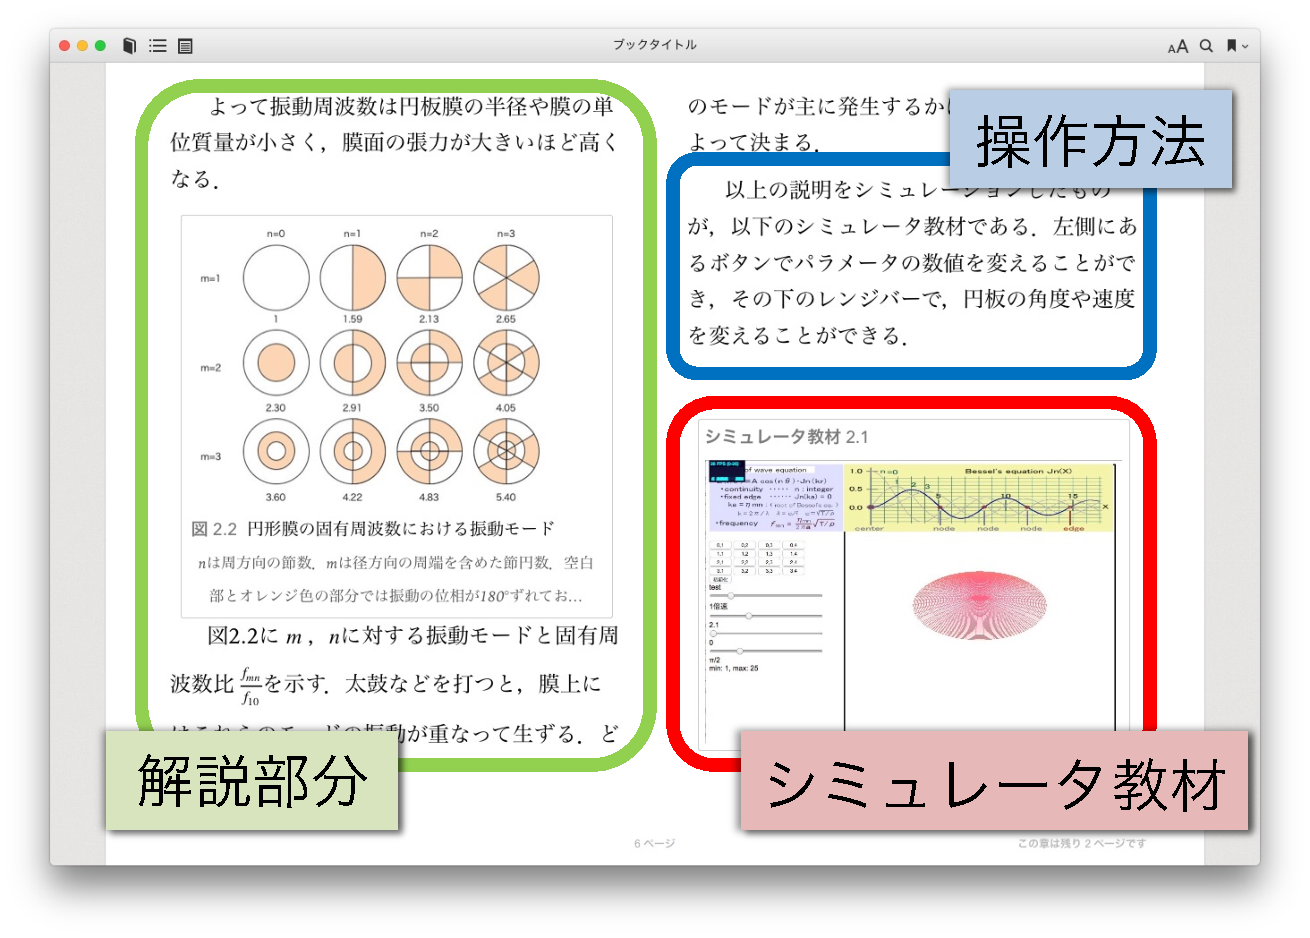
\includegraphics[clip,width=85mm,height=55mm]{textbook.pdf}
\end{center}
 \caption{電子教科書サンプル}
 \label{fig:教科書}
\end{figure}

\section{やること・やったこと}

論文や書籍から,ゲームで行われるグラフィックなどの処理を学び,開発を行うベンチマークソフトの参考とする.


\section{今後の予定}
Unityで,ゲームと同様の処理を行えるソフトの開発を行う

\begin{thebibliography}{99}
\bibitem{1} 須田宇宙: ``音響科学e-Learning教材'', \url{https://www.youtube.com/watch?v=rZdvL0ju4CA&ab_channel=TheSpyHood}, 2018/7/19参照
\end{thebibliography}

\end{document}
